%\placelogofalse
\begin{frame}{Incremental Partition Maintenance}
\begin{columns}
\column{0.58\linewidth}
\centering
\begin{outline}
  \1 Maintenance actions
  \2 Split Partition
  \2 Merge Partition
  \2 Add Level (top)
  \2 Remove Level (top)
\end{outline}

\column{0.38\linewidth}
\begin{center}
\centering
%\shadowimage[width=2.5cm]{example_1.png}

%\includegraphics[width=2.5cm]{example_3.png}

% [trim={left bottom right top},clip]
%\includegraphics[width=8.5cm, page=3, trim={0 9cm 14cm 0cm},clip]{assets/vec_db_figs.pdf}
\end{center}
\end{columns}

\vspace{0.2cm}

\begin{center}
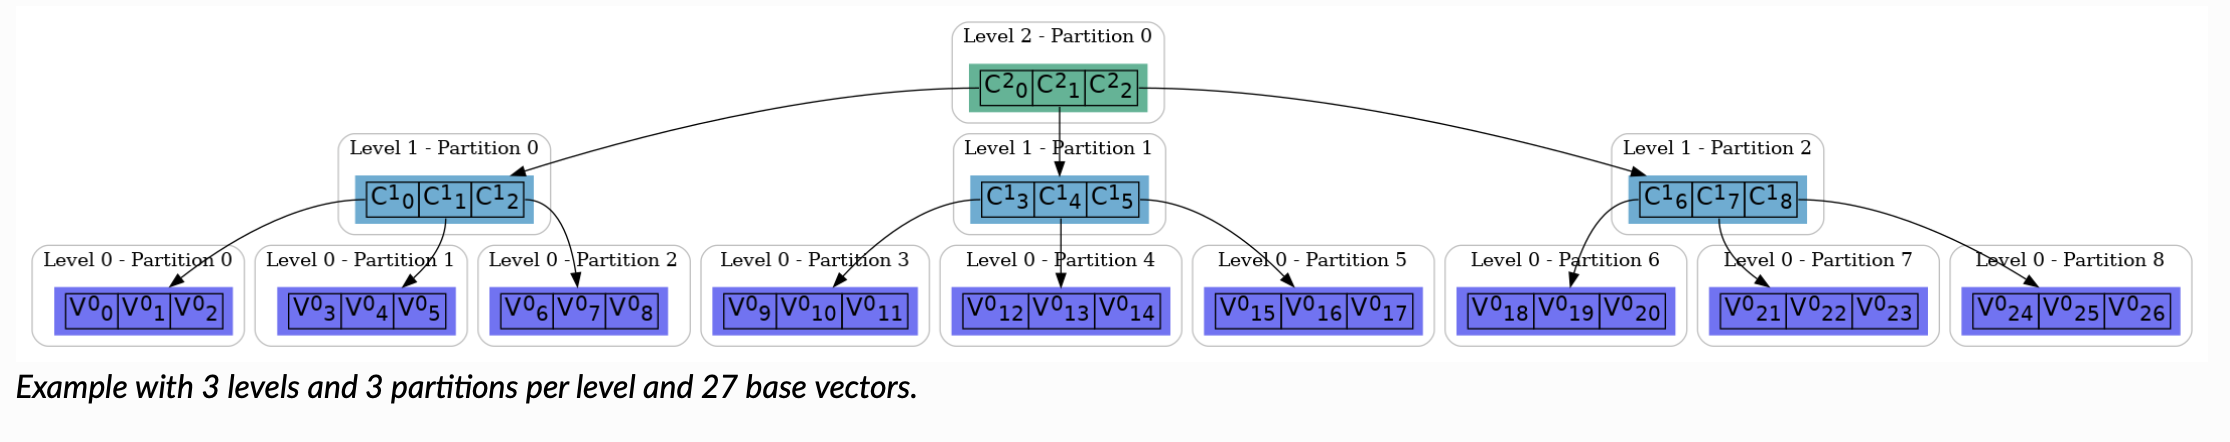
\includegraphics[width=11.0cm]{assets/data_layout.png}

{\tiny From \href{https://marius-project.org/quake/architecture/architecture.html}{Quake Documentation}}
\end{center}
\end{frame}
%\placelogotrue

%\placelogofalse
\begin{frame}{Cost-Driven Maintenance}
Use a cost-model for query latency to determine which partitions to split / merge.
\begin{columns}
\column{0.48\linewidth}
\begin{align*}
  C &= \sum_{i}C_i \ \text{Total cost (latency)}\\
  C_i &= O_c + A_i \lambda(s_i) \ \text{Per-partition cost}\\
\end{align*}
\column{0.48\linewidth}
\begin{align*}
  A_i & \ \text{Access frequency of partition }i \\
  s_i & \ \text{Size of partition }i \\
  \lambda(s_i) & \ \text{Latency to scan partition } i \\
O_c & \ \text{Latency to scan centroid}
\end{align*}
\end{columns}
Estimate the change in cost of a split / merge, take action if expected to reduce cost
$$
\Delta C_i = c_i + \Delta{\text{split}_i} \ \ \text{If} \ \Delta C_i < \tau \ \text{then split partition } i
$$
\end{frame}
%\placelogotrue
